% This file was created with tikzplotlib v0.9.12.
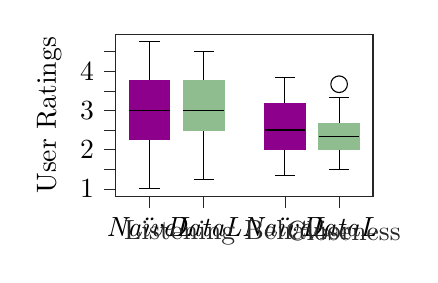
\begin{tikzpicture}

\definecolor{color0}{rgb}{0.254901960784314,0.411764705882353,0.882352941176471}
\definecolor{color1}{rgb}{0.941176470588235,0.501960784313725,0.501960784313725}


%\definecolor{color0}{rgb}{0.34, 0.01, 0.1} %0 - very dark pink
\definecolor{color0}{rgb}{0.91, 0.59, 0.48} %1 - light salmon
%\definecolor{color0}{rgb}{0.09, 0.45, 0.27} %4  - lighter green
\definecolor{color1}{rgb}{0.56, 0.74, 0.56} %5 - very light green
\definecolor{color0}{rgb}{0.53, 0.15, 0.34} %2 --dark pink
%\definecolor{color1}{rgb}{0.18, 0.31, 0.31} %3 --- dark green
\definecolor{color0}{rgb}{0.45, 0.31, 0.59} %new color 0
\definecolor{color0}{rgb}{0.59, 0.44, 0.84} %new color1
%\definecolor{color0}{rgb}{0.55, 0.0, 0.55} %new color 2
\definecolor{color0}{rgb}{0.55, 0.0, 0.55} %new color 2

%[group style={group size=1 by 2},width=0.4\textwidth, height=0.25\textwidth, legend style={nodes={scale=0.8, transform shape}},
\begin{axis}[
axis line style={white!15!black},
tick align=outside,
tick pos=left,
x grid style={white!80!black},
xmin=-0.4, xmax=3.4,
xtick style={color=white!15!black},
xtick={0.1,0.9,2.1,2.9},
xticklabels={\textit{NaïveL},\textit{DataL},\textit{NaïveL},\textit{DataL}},
y grid style={white!80!black},
ylabel={User Ratings},
ymin=0.8125, ymax=4.9375,
ytick style={color=white!15!black},
ytick={1,1.5,2,2.5,3,3.5,4,4.5,5},
yticklabels={1,,2,,3,,4,,5},
width=0.4\textwidth, height=0.3\textwidth, clip=false
]
\addplot [black]
table {%
0.1 2.25
0.1 1
};
\addplot [black]
table {%
0.1 3.75
0.1 4.75
};
\addplot [black]
table {%
-0.05 1
0.25 1
};
\addplot [black]
table {%
-0.05 4.75
0.25 4.75
};
\addplot [black]
table {%
0.9 2.5
0.9 1.25
};
\addplot [black]
table {%
0.9 3.75
0.9 4.5
};
\addplot [black]
table {%
0.75 1.25
1.05 1.25
};
\addplot [black]
table {%
0.75 4.5
1.05 4.5
};
\addplot [black]
table {%
2.1 2
2.1 1.33333333333333
};
\addplot [black]
table {%
2.1 3.16666666666667
2.1 3.83333333333333
};
\addplot [black]
table {%
1.95 1.33333333333333
2.25 1.33333333333333
};
\addplot [black]
table {%
1.95 3.83333333333333
2.25 3.83333333333333
};
\addplot [black]
table {%
2.9 2
2.9 1.5
};
\addplot [black]
table {%
2.9 2.66666666666667
2.9 3.33333333333333
};
\addplot [black]
table {%
2.75 1.5
3.05 1.5
};
\addplot [black]
table {%
2.75 3.33333333333333
3.05 3.33333333333333
};
\addplot [black, mark=o, mark size=3, mark options={solid,fill opacity=0}, only marks]
table {%
2.9 3.66666666666667
};
\path [draw=color0, fill=color0]
(axis cs:-0.2,2.25)
--(axis cs:0.4,2.25)
--(axis cs:0.4,3.75)
--(axis cs:-0.2,3.75)
--(axis cs:-0.2,2.25)
--cycle;
\path [draw=color1, fill=color1]
(axis cs:0.6,2.5)
--(axis cs:1.2,2.5)
--(axis cs:1.2,3.75)
--(axis cs:0.6,3.75)
--(axis cs:0.6,2.5)
--cycle;
\path [draw=color0, fill=color0]
(axis cs:1.8,2)
--(axis cs:2.4,2)
--(axis cs:2.4,3.16666666666667)
--(axis cs:1.8,3.16666666666667)
--(axis cs:1.8,2)
--cycle;
\path [draw=color1, fill=color1]
(axis cs:2.6,2)
--(axis cs:3.2,2)
--(axis cs:3.2,2.66666666666667)
--(axis cs:2.6,2.66666666666667)
--(axis cs:2.6,2)
--cycle;
\addplot [black]
table {%
-0.2 3
0.4 3
};
\addplot [black]
table {%
0.6 3
1.2 3
};
\addplot [black]
table {%
1.8 2.5
2.4 2.5
};
\addplot [black]
table {%
2.6 2.33333333333333
3.2 2.33333333333333
};
\draw (axis cs:-0.42, -0.12) node[
  %scale=1.5,
  anchor=west,
  text=white!15!black,
  rotate=0.0
]{Listening Behavior};
\draw (axis cs:1.98,-0.08) node[
  %scale=1.5,
  anchor=west,
  text=white!15!black,
  rotate=0.0
]{Closeness};
\end{axis}

\end{tikzpicture}
